\documentclass[12pt,a4paper,onecolumn,titlepage]{report}

%%%%%%%%%%%%%%%%%%%%%%%%%%%%%%%%%%%%%%%%%
%UMLAUTS TO WORK CORRECTLY IN BIBLIOGRAPHY
%%%%%%%%%%%%%%%%%%%%%%%%%%%%%%%%%%%%%%%%%
\PassOptionsToPackage{backend=biber}{biblatex}
\usepackage[T1]{fontenc}    % font type
\usepackage[utf8]{inputenc} % western european alphanumerics?
\usepackage{cite}
%%%%%%%%%%%%%%%%%%%%%%%%%%%%%%%%%%%%%%%%%



%%%%%%%%%%%%%%%%%%%%%%%%%%%%%%%%%%%%%%%%%
%MATHS PACKAGES
%%%%%%%%%%%%%%%%%%%%%%%%%%%%%%%%%%%%%%%%%
\usepackage{siunitx}
\usepackage{amsmath} 
\usepackage{bm}% bold math
%%%%%%%%%%%%%%%%%%%%%%%%%%%%%%%%%%%%%%%%%



%%%%%%%%%%%%%%%%%%%%%%%%%%%%%%%%%%%%%%%%%
%PAGE LAYOUT
%%%%%%%%%%%%%%%%%%%%%%%%%%%%%%%%%%%%%%%%%
% em = width of a capital letter in the designated font
\usepackage[margin=3cm,footskip=2.0cm,top=2cm,bottom=2cm]{geometry}
\setlength{\parindent}{0cm} % paragraph initial indentation
\setlength{\parskip}{1em}   % paragraph separation
\renewcommand{\baselinestretch}{1.5} % character spacing?
\pagestyle{headings}        % format of the pages
%\usepackage{helvet}
%\renewcommand{\familydefault}{\sfdefault}
\usepackage[UKenglish]{isodate}

\usepackage{hyperref}       % clickable references and figures
\hypersetup{colorlinks=true, citecolor=blue, urlcolor=blue, linkcolor=black} % colour your \refs
\usepackage{listings}% for code blocks
%\usepackage{lipsum}% generates filler text

%verbatim remove whitespace
\usepackage{etoolbox}
\makeatletter
\preto{\@verbatim}{\topsep=0pt \partopsep=0pt }
\makeatother
%%%%%%%%%%%%%%%%%%%%%%%%%%%%%%%%%%%%%%%%%



%%%%%%%%%%%%%%%%%%%%%%%%%%%%%%%%%%%%%%%%%
%GRAPHICS LOCATION AND PACKAGES (CAPTION)
%%%%%%%%%%%%%%%%%%%%%%%%%%%%%%%%%%%%%%%%%
\usepackage{graphicx}           % graphics package to use
\graphicspath{ {DGraphics/} }   % folder name where graphics are located
\usepackage{caption}            % caption formatting package
\captionsetup[subfigure]{position=top,singlelinecheck=off,justification=raggedright}
\usepackage{subfig}             % allow subfigures to work
\usepackage{wrapfig}            % formats how text wraps around figure

\usepackage{relsize}            % makes table references smaller
\usepackage{multirow}           % allows extra rows in figures
\usepackage{dcolumn}            % Align table columns on decimal point
\usepackage{hhline}
%%%%%%%%%%%%%%%%%%%%%%%%%%%%%%%%%%%%%%%%%



%%%%%%%%%%%%%%%%%%%%%%%%%%%%%%%%%%%%%%%%%
%CHAPTER PAGE SETTINGS
%%%%%%%%%%%%%%%%%%%%%%%%%%%%%%%%%%%%%%%%%
%sets up the first page of each chapter
\makeatletter
\renewcommand\chapter{\if@openright\cleardoublepage\else\clearpage\fi
                    \thispagestyle{empty}%
                    \global\@topnum\z@
                    \@afterindentfalse
                    \secdef\@chapter\@schapter}
\makeatother
%%%%%%%%%%%%%%%%%%%%%%%%%%%%%%%%%%%%%%%%%



%%%%%%%%%%%%%%%%%%%%%%%%%%%%%%%%%%%%%%%%%
%NEW COMMANDS
%%%%%%%%%%%%%%%%%%%%%%%%%%%%%%%%%%%%%%%%%
\newcommand{\subfigref}[2][\figurename~]{#1\ref{#2}}
\newcommand{\figref}[2][Figure ]{#1\ref{#2}}
\newcommand{\tabref}[2][Table ]{#1\ref{#2}}
\newcommand{\secref}[2][Section~]{#1\ref{#2}}

\newcommand{\code}[2][]{\texttt{#2}}
\newcommand{\codeinline}[2][]{{\tt#2}}
\newcommand{\codeline}[2][]{\hspace{2em}{\tt#2}}
\newcommand{\etal}{\emph{et al.}}
\newcommand{\abinitio}{\emph{ab initio}}
\newcommand{\artemis}{{ARTEMIS}}
%%%%%%%%%%%%%%%%%%%%%%%%%%%%%%%%%%%%%%%%%



\begin{document}
\begin{titlepage}
\pagenumbering{gobble}     % gobbles up (remove/eats up) the page number for this page 
\title{\center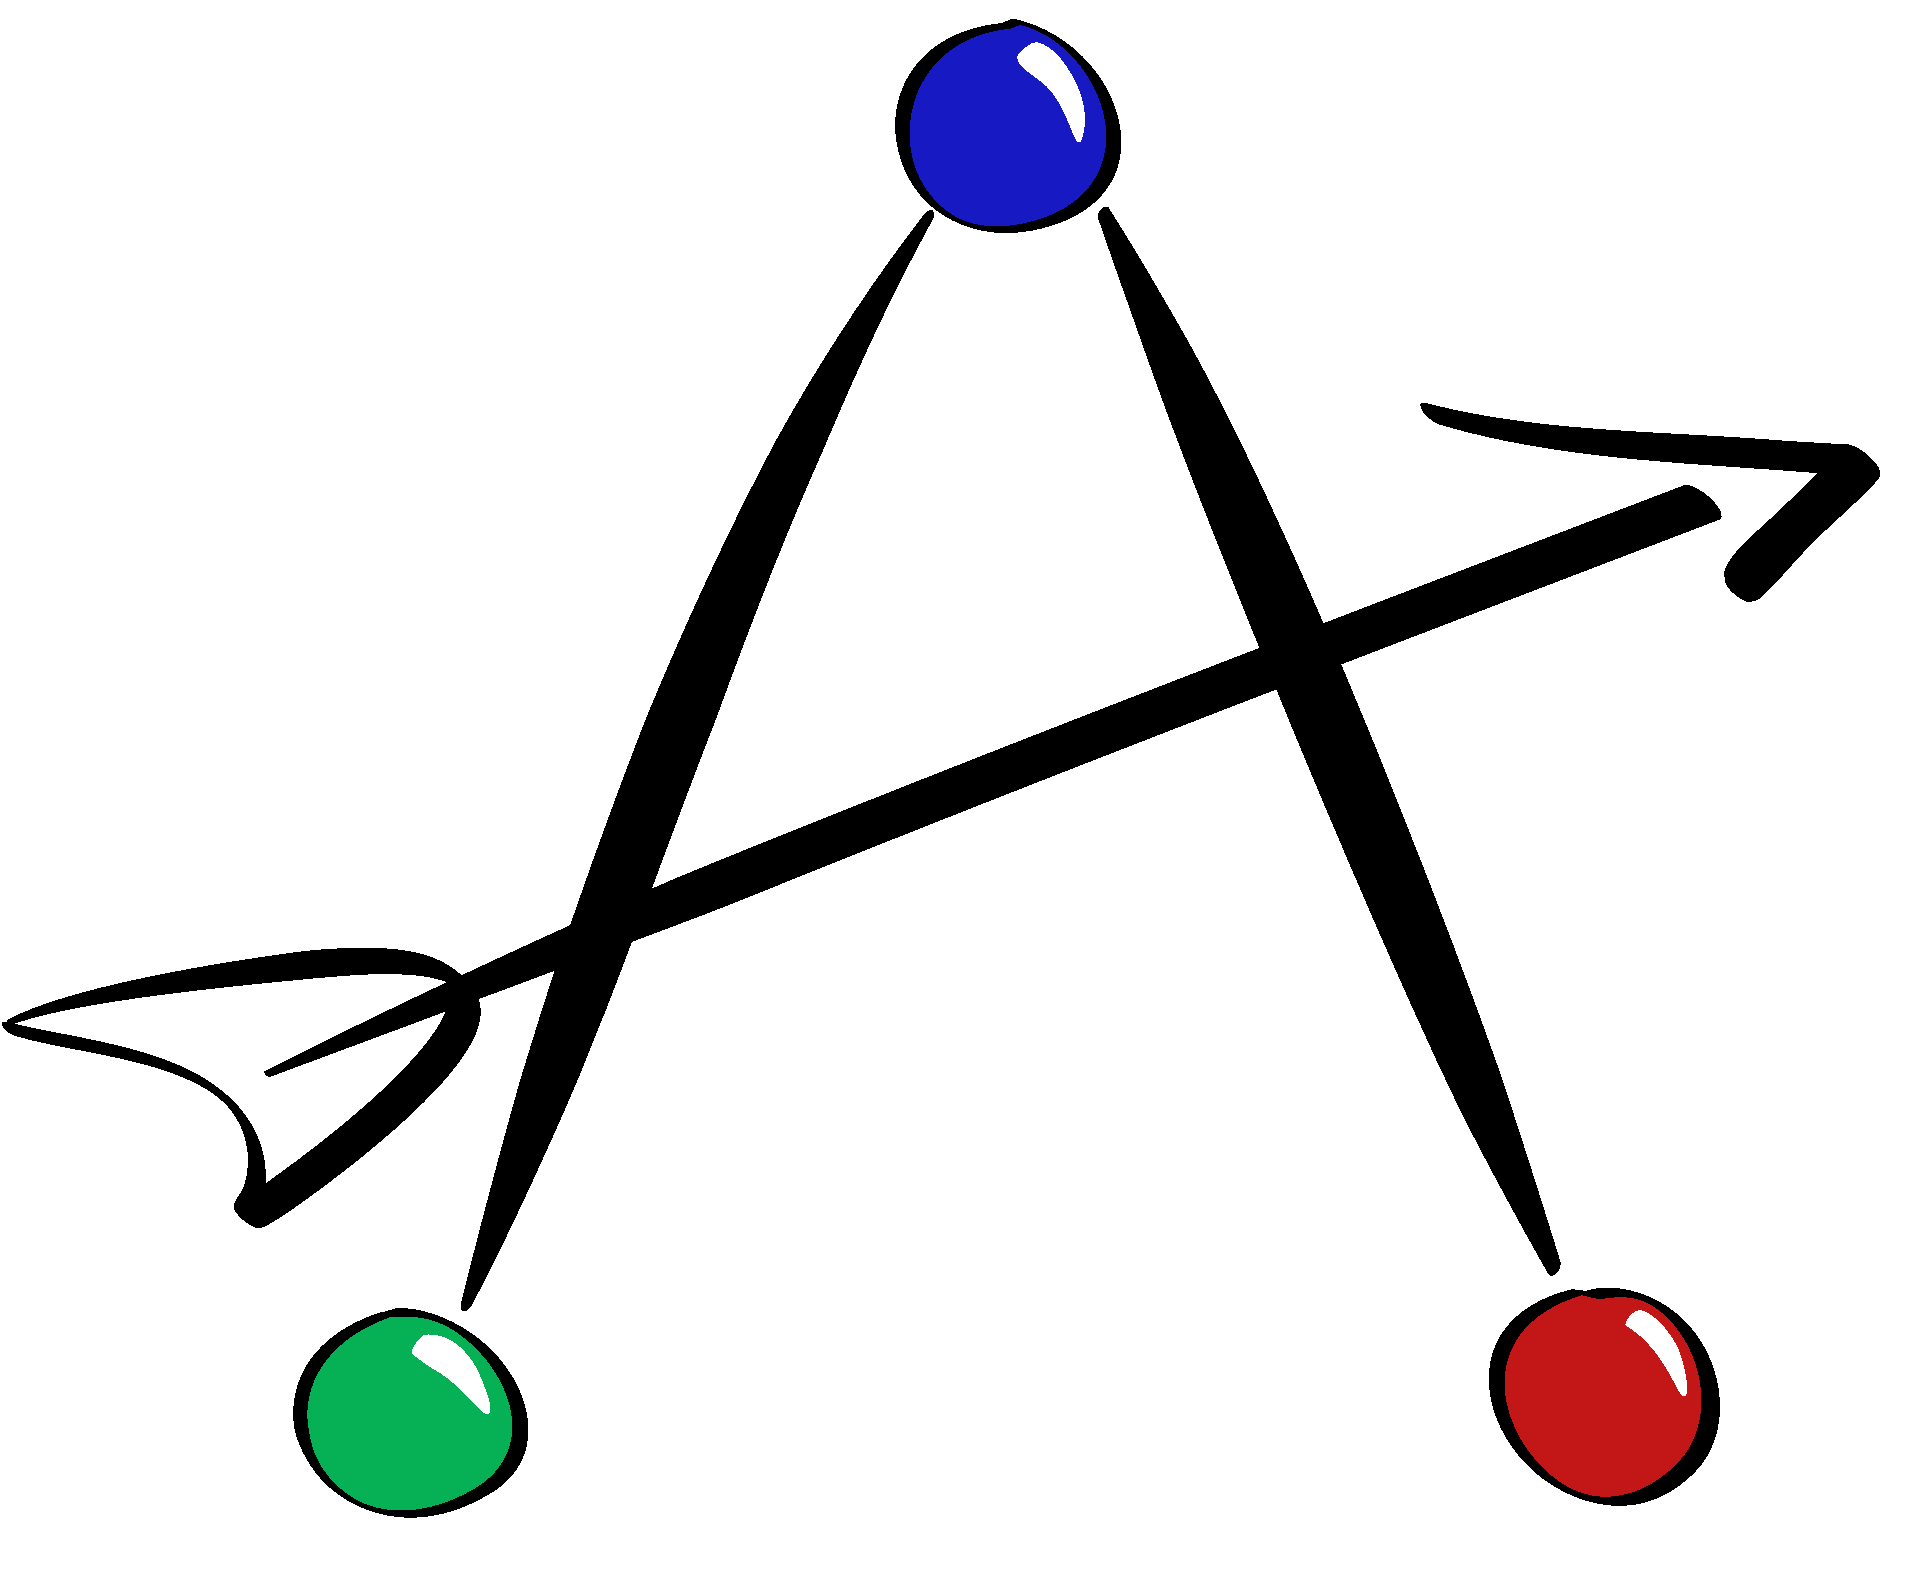
\includegraphics[scale=0.25]{../artemis_logo.pdf}\\{\emph{Ab initio}} Restructuring Tool Enabling the Modelling of Interface Structures (ARTEMIS): A User Guide}
\author{Ned Thaddeus Taylor}
\date{\today}
%\onecolumn	% makes title and abstract appear over entire page width
\maketitle % formats the title
\end{titlepage}



\pagenumbering{arabic}

\newpage
\setcounter{page}{2}  % resets the page number
\tableofcontents
\newpage



\chapter{Features/Capabilites}

\artemis{} is a tool intended to help users with interface generation. Here is a list of the features it currently supports:

\begin{itemize}
\item Read and write geometry structure files of the formats used by VASP, CASTEP and Quantum Espresso. 
\item Generate slabs along user-defined Miller planes (generates all possible surface terminations in this plane)
\item Determine lattice matches within defined strain tolerances for two parent structures given by the user and generate interfaces based on these.
\item Determine the primitive layer of the parent structures and use these to build the parent regions of the interface structures to user-defined thicknesses.
\item Identify unique surface terminations for structures along user-defined Miller planes and print slabs of these for the user to study.
\item Identify unique terminations of the parent structures for Miller planes and use these to generate unique interfaces with these being the surfaces at the interface.
\item Generate unique interface shifts to allow the user to explore the energetic space of interfacial alignment.
\item Generate unique interface swaps (intermixing) to allow the user to explore graded interfaces.
\item Take in pregenerated interface structures and determine the location of their interfaces.
\item Take in pregenerated interface structures and perform shifts and swaps on them to generate further potential interfaces.
\end{itemize}


\chapter{Credits and Licence}

\section{Credits}
\label{sec:credits}

The \artemis{} code was developed by Ned Thaddeus Taylor and Steven Paul Hepplestone. Many of the subroutines and functions used by the code were developed by Ned Thaddeus Taylor and Francis Huw Davies. During his Summer project, Isiah Edward Mikel Rudkin worked alongside Ned to develop the shifting and swapping modules of \artemis{}, along with helping test the code.

For further information about the group behind \artemis{}, follow the link \url{http://www.artemis-materials.co.uk/}.

For support and sending bug-reports, please contact the following email address:
\noindent
\codeinline{support@artemis-materials.co.uk}




\section{Licence}
\label{sec:licence}

This work is licensed under a Creative Commons Attribution-NonCommercial 3.0 Unported (CC BY-NC 3.0) License (\url{https://creativecommons.org/licenses/by-nc/3.0/}). Please refer to the link for a detailed description of the license.

\begin{figure}[h]{}

\includegraphics[scale=0.1]{Cc-by-nc_icon.png}\label{fig:cc}
\end{figure}

\section{Beta testers}
\label{sec:testers}

The following people have engaged in useful discussions that have helped to improve the quality of the program and have tested it to help find bugs in the software.

\begin{enumerate}
\item Conor Jason Price (University of Exeter)
\item Tsz Hin Chan (University of Exeter)
\item Joe Pitfield (University of Exeter)
\item Edward Allery David Baker (University of Exeter)
\item Shane Graham Davies (University of Exeter)
\end{enumerate}


\chapter{Getting started}

\section{Requirements}
\label{sec:req}

The following utilities are required to install \artemis{}:

\begin{itemize}
\item gcc version 7.2.0 (GNU Compiler Collection). Type \codeinline{gcc -{}-version} to verify this. This package can be downloaded from \url{https://gcc.gnu.org/}
\item GNU make (any version). Type \codeinline{make -{}-version} to verify this. This package can be downloaded from \url{https://gcc.gnu.org/}
\end{itemize}

ARTEMIS has currently been tested to work using both the gcc fortran compiler mentioned above and the Intel fortran compiler (ifort version 17.0.4). Keep in mind, though, that ARTEMIS has been developed using the gcc fortran compiler and, as such, has been more thoroughly tested using this compiler. Whilst compilation should work with newer versions of the compilers, this has not been tested.

ARTEMIS is known to not compile with gcc version 4.8.0. This is due to that version not supporting the \codeinline{allocate(MATRIX,source=SOURCE)} and the \codeinline{movealloc()} Fortran built-in subroutines.


You may also want a first-principles electronic structure calculation code in order to make use of the output structures to determine the energetics of them.


\section{Installation}
\label{sec:install}

Type
\codeline{tar -xvzf ARTEMIS\_X.X.X.tar.gz}

\noindent
where \codeinline{X.X.X} is the current version number. This command creates a directory called \codeline{DARTEMIS} in the current directory which contains the whole software package. From now on, I will refer to the access path to this directory as \codeinline{DARTEMIS}.

Type 
\codeline{cd DARTEMIS}

\noindent
By default, when making \artemis{}, it will output the executable into a \codeinline{bin} directory in \codeinline{DARTEMIS}. The user can change where the executable is compiled by editing the Makefile line \codeinline{BIN\_DIR := ./bin} in \codeinline{Makefile} to point to the location where the execultable is wanted. Type

\codeline{make}

\noindent
This should compile the code into an executable called \codeinline{artemis} in the designated bin directory. We highly recommend that the user copies this executable into their \codeinline{\$(HOME)/bin} directory and the manual assumes from now on that the user has done so (if not done, then whenever \codeinline{artemis} is seen in the manual, replace this with the filepath to the \codeinline{artemis} executable).


\section{Test ARTEMIS with a simple example}
\label{sec:test_case}

In the \codeinline{artemis} directory, three examples highlighting the use of \artemis{} can be found in the \codeinline{examples} subdirectory. The three presented examples are for generating new interfaces (\codeinline{generate\_interface} directory) and manipulating pregenerated interfaces (\codeinline{pregenerated\_interface} directory) and exploring all unique surface terminations of slabs (\codeinline{identify\_terminations}).

\subsection{Generate interface example}
\label{sec:example_gen}

Change to the \codeinline{generate\_interface} directory and type

\codeline{artemis -f param.in}

\noindent
\artemis{} will then read the \codeinline{param.in} file and set the parameters as defined in there for the run. A directory named \codeinline{DINTERFACES} will then be generated and populated with directories and structure files. As defined by the parameter file, \codeinline{POSCAR\_Si} and \codeinline{POSCAR\_Ge} are used for the two parent structure files.

This example is set up to show how \artemis{} can find matched between two materials and perform shifts and swaps based on these generated interface structures.


\subsection{Pregenerated interface example}
\label{sec:example_pregen}

Change to the \codeinline{pregenerated\_interface} directory and type

\codeline{artemis -f param.in}

\noindent
\artemis{} will then read the \codeinline{param.in} file and set the parameters as defined in there for the run. A directory named \codeinline{DINTERFACES} will then be generated and populated with directories and structure files.

This example is set up to show how \artemis{} can determine the location of interfaces within a structure and can use that information to perform additional shifts and swaps to allow the user to further explore the energetic space of the interface.


\subsection{Identify terminations example}
\label{sec:example_terms}

Change to the \codeinline{identify\_terminations} directory and type

\codeline{artemis -f param.in}

\noindent
\artemis{} will then read the \codeinline{param.in} file and set the parameters as defined in there for the run. A directory named \codeinline{DTERMINATIONS} will be made with a \codeinline{DLW\_TERMS} directory (and \codeinline{DUP\_TERMS}, if \codeinline{STRUC2\_FILE} and \codeinline{UP\_MILLER} are defined) inside. This directory will contain the unique surface termination slab structures.

This example is set up to show how \artemis{} can generate slabs cleaved along user-defined Miller planes. In such a case, it will determine all unique surface terminations in that plane and print them to files termed as \codeinline{POSCAR\_term\{1..n\}}, where \codeinline{n} is the number of unique surface terminations identified by \artemis{}.



\chapter{Version History}

Format is based on [Keep a Changelog] (\url{https://keepachangelog.com/en/1.0.0/}),
and this project adheres to [Semantic Versioning](https://semver.org/spec/v2.0.0.html).

\begin{verbatim}
## [Alpha 1.0.0] - 2019-05-31
### Added
- Changelog introduced
- IMATCH 0, 1 and 2
- ISHIFT 0, 1 and 2
- Symmetry checks performed over matches

### Changed
- Source code moved to src/ and Makefile compiles from ./
- Updated default infile that is generated to include new opptions


## [Beta 1.0.0] - 2019-11-28
### Added
- IMATCH 3 and 4
- ISHIFT 3 and 4
- Help and search function

### Changed
- LREDUCE default changed from TRUE to FALSE


## [Beta 1.1.0] - 2019-12-18
### Added
- LW_SURFACE, UP_SURFACE
-- user-defined surface terminations
- LW_LAYERED, UP_LAYERED
-- user defines whether material is layered


## [Public release 1.0.0] - 2020-02-26
### Added
- TOL_SYM
-- user-defined symmetry precision/tolerance
- ISWAP method 2
-- method weights swapping based on distance from interface
- Restart job prints out interface location for use by user
- Optional user defined interface location - for restart
- SWAP_DENSITY allows for consistency of swapping concentration over
  structures
- User manual (doc/manual.pdf)
- LMIRROR added for swapping
-- says whether to maintain symmetry of interfaces or to perform 
   swaps on one
-- only listened to if interfaces are not symmetric
- Added support email address to README and manual
- Added date of compilation to code
- Added date of execution of code to the output
- Added make install to build ARTEMIS executable 
  in $(HOME)/bin directory
- Added make uninstall to remove ARTEMIS executable 
  from $(HOME)/bin directory
- Added help for OUTPUT_FILE tag in CELL_EDITS card
- Added help for LSURF_GEN tag ino CELL_EDITS card
- ISHIFT=4 method updated
-- DON for upper parent crystal is now scaled appropriately the same
   as the lattice is
-- reduces issue of DONs finding more bonds at the surface than in
   the bulk
-- Update appears in interfaces.f90 gen_interfaces subroutine
- Added LAYER_SEP flag to CELL_EDITS card
-- need to figure out solution for shared cards
- Added help for LORTHO tag in CELL_EDITS and INTERFACES cards
-- defines whether surface axis is orthogonal when using LSURF_GEN
- Added example runs input/output files and input structures
-- example for detecting pregenerated interfaces
-- example for generating new interfaces
-- example for surface generation

### Changed
- Makefile now defaults to compiling executable into user's home bin
- LREDUCE default now FALSE
- Changed io.f90 to io.F90 to allow for preprossing of file
-- now includes date of compilation
- Settings output file now contains more of the important tags
- Changed make clean to remove bin/ and obj/ directories 
  in the ARTEMIS directory
- f_scale and g_scale are now global variables
  in mod_shifting.f90 for ISHIFT=4
- Changed OUTFILE tag to OUTPUT_FILE
- Changed LSURF_GEN tag help description
- STRUC2_FILE no longer a mandatory tag for all cases
-- no longer required for LSURF_GEN = TRUE
-- no longer required for TASK = 0

### Removed
- LSWAP replaced with ISWAP
-- LSWAP = F is now ISWAP = 0
-- LSWAP = T is now ISWAP = 1
- NSWAP replaced with SWAP_DENSITY
- NSWAP_OUT replaced with NSWAP
- LSURF_INFO replaced with LSURF_GEN in INTERFACES card

### Fixed
- Unique termination identifier
-- inversion symmetry matches
-- reset symmetry list after each save
- Layer identification
- basis_map subroutine in mod_sym
- Correctly print and define vector mismatch to be maximum mismatch 
  of any one vector
- Correctly convert symmetries to new lattice space for use in 
  mod_plane_matching.f90 and mod_lat_compare.f90
- Fixed area mismatch value printing
- Works again with Intel fortran compiler ifort 17.0.4
- Fixed denominator of ISHIFT g function
-- now normalises to bond size
- Corrected help function for LREDUCE default to FALSE
- Fixed termination idenitifier again
-- works correctly for slabs without mirror symmetry now with ladders
- Fixed error in mod_plane_matching.f90
-- did not correctly save the smallest area lattice match with the 
   same symmetry
- No longer makes DINTERFACES directory when not necessary
-- e.g. does not make it when generating surfaces


## [Public release 1.0.1] - 2020-05-04

### Added
- added gen_group function into mod_misc_linalg.f90 to generate entire
  group from a subset of elements
-- used in the updated version of the setup_ladder subroutine.

### Fixed
- setup_ladder subroutine
-- now correctly identifies the separation between identical layers for
   systems with both mirrored and translation symmetries transforming
   between layers


\end{verbatim}



\chapter{User guide}

\section{Input files}
The \artemis{} code needs either two or three input files: one that provides the parameters to guide the interface generation and either one or two files that specify the geometries of the parent structure/structures. If the user intends to use a pregenerated interface and manipulate this structure, then only one geometry parent file is required. If one wants to generate a set of interfaces from the combination of two parent structures, then two geometry parent files are required (one for each of the parent structures). The geometry file formats currently supported include: VASP, CASTEP, Quantum Espresso. For an example of the parameters file, running the following command will generate such a file:

\codeline{artemis -d param.in}

\noindent
This will generate an input file with some of the tags/parameters present. The input file is structured in the following way:

\begin{tabular}{p{\linewidth}}
\hline
\vspace{-1em}
\begin{verbatim}
SETTINGS        (beginning of settings card)
  TAG = 
END SETTINGS    (end of card)

INTERFACES      (beginning of interface card)
  TAG = 
END INTERFACES  (end of interface card)
\end{verbatim}
\tabularnewline [-2em]
\hline
\end{tabular}

\noindent
where the cards separate blocks of the parameters that are distinct in their actions. Cards are started by a \code{CARDNAME} and ended when met with \code{END[ ]CARDNAME}. Tags/parameters are found within these tags and are used to alter the settings of the run. For an brief description of each of the tags available within each card, type

\codeline{artemis --help all}

\noindent
This displays a list of all tags currently available within \artemis{}, with a brief description of their use. To get a more indepth description of each one, type

\codeline{artemis --help <TAGNAME>}

\noindent
where \code{<TAGNAME>} is the name of the tag that the user wants to know more about. If the user wants to find all tags relating to a certain word, then type

\codeline{artemis --search <WORD>}

\noindent
All tags that include this word will be printed to the terminal.

The one/two parent geometry files are specified using the following tags in the \code{SETTINGS} card:

\begin{tabular}{p{\linewidth}}
\hline
\vspace{-1em}
\begin{verbatim}
SETTINGS
  STRUC1_FILE = <PARENT_FILE_1>
  STRUC2_FILE = [PARENT_FILE_2]
END SETTINGS
\end{verbatim}
\tabularnewline [-2em]
\hline
\end{tabular}



\section{Running the code}
\label{sec:run_code}

Once the input files have been gathered, \artemis{} can be run by entering the command

\codeline{artemis -f [INPUT\_FILENAME]}

\noindent
where the flag \codeinline{-f} takes [INPUT\_FILENAME] as the input file and runs the code using the parameters specified in that file.

Once this has been run, a directory tree will be generated, depending on the options ran with. When generating interfaces, the \codeinline{DINTERFACES/} directory will be made. When surface terminations are requested (\code{LSURF\_INFO}, default = False), then \codeinline{DTERMINATIONS/} will be made. Inside these directories, a directory tree containing the output structure files will be generated.




\section{Outputs of ARTEMIS}
\label{sec:outputs}

Here is an example output directory tree generated by \artemis{}. In this example, \code{NSHIFT} = 2 and \code{NSWAP} = 2, and the output file format of VASP has been used. For each unique interface match and termination, a directory in \code{DINTERFACES/} will be generated, with the form \code{D01/}, \code{D02/}, \code{D03/}, etc. Inside each of these, shifts of the generated interface match will be made and placed inside \code{DSHIFTS}. And inside each of those, any requested swaps will populate the \code{DSWAPS} directory.

\begin{tabular}{p{\linewidth}}
\hline
\vspace{-1em}
\begin{verbatim}
|- DINTERFACES/
|  |- D01/
|  |  |- DSHIFTS/
|  |  |  |- D01/
|  |  |  |  |- POSCAR
|  |  |  |  |- DSWAPS/
|  |  |  |  |  |- D01/
|  |  |  |  |  |  |- POSCAR
|  |  |  |  |  |- D02/
|  |  |  |  |  |  |- POSCAR
|  |  |  |- D02/
|  |  |  |  |- POSCAR
|  |  |  |  |- DSWAPS/
|  |  |  |  |  |- D01/
|  |  |  |  |  |  |- POSCAR
|  |  |  |  |  |- D02/
|  |  |  |  |  |  |- POSCAR
|  |- D02
...
\end{verbatim}
\tabularnewline [-2em]
\hline
\end{tabular}



\section{Conclusion}

The \artemis{} code is intended to help the user more easily and quickly explore the possibility space of interfaces between two materials. With its ability to determine lattice matches, perform shifts and swaps, this should help reduce potential bias that can be associated with such a problem by making it easier to create these interfaces. This should enable users to focus more heavily on the idea of interfacial aligment and give them the ability to explore the problem of interfaces with more ease.


%\bibliography{}


\end{document}
